\documentclass{standalone}

\usepackage[english]{babel}
\usepackage[linesnumbered, ruled, vlined]{algorithm2e}

\usepackage{caption}

% to create listings

\usepackage{listings, lstautogobble}
\lstset{
  autogobble=true,
  frame=single,
}

\lstdefinelanguage{coq}[Objective]{Caml}{
  morekeywords={Structure, Definition, Inductive, list, return},
  sensitive=true
}

% to define font size

\usepackage{ulem}
\usepackage{moresize}
\usepackage{anyfontsize}

% to use tikz and its libraries

\usepackage{tikz-timing}
\usepackage{tikz}

\usetikzlibrary{backgrounds}
\usetikzlibrary{decorations.pathreplacing, positioning, calc, arrows, shapes, automata, petri, patterns}
\usetikzlibrary{decorations.markings}

% to use tikzmark, to place and refer to marks outside the current figure

\tikzset{every picture/.style={remember picture}}

% styles for transitions

\tikzset{transition/.append style={fill=black!20, thick}}
\tikzset{transition/.append style={fill=black!20, thick}}

% styles for test and inhib arcs.

\tikzstyle{test}=[pre, *-]
\tikzstyle{inhib}=[pre, o-]

% Arrow positioning in a path

\tikzset{->-/.style={decoration={
  markings,
  mark=at position #1 with {\arrow{>}}},postaction={decorate}}}

\tikzset{-<-/.style={decoration={
  markings,
  mark=at position #1 with {\arrow{<}}},postaction={decorate}}}

% to use colors

\usepackage{xcolor}

%%%%%%%%%%%%%%%%%%%%%%%%%%%%%%%%%%%%%%%%%%%%%%%%%%
%                  BEGIN DOCUMENT                %
%%%%%%%%%%%%%%%%%%%%%%%%%%%%%%%%%%%%%%%%%%%%%%%%%%

\begin{document}

\begin{tikzpicture}


  \node (pn) {
    \begin{tikzpicture}

      % PLACES AND TRANSITIONS
      
      \node[place,tokens=1] (p0) {};
      
      \node[transition] (t0) at ($(p0)-(0,1)$) {};
      
      \node[place] (p1) at ($(t0)-(0,1)$) {};

      \node[transition] (t1) at ($(p1)-(0,1)$) {};

      % LABELS

      \node (pzLabel) at ($(p0)-(.7,-.2)$) { $p_0$};
      \node (tzLabel) at ($(t0.west)-(.3,-.2)$) {$t_0$};
      \node (poLabel) at ($(p1)-(.7,0)$) { $p_1$};
      \node (tzLabel) at ($(t1)-(.5,.2)$) { $t_1$};

      % ACTIONS, FUNCTIONS, CONDITIONS AND TIME ITVALS

      \node (a0) at ($(p0.east)+(.3,0)$) {$a_0$};
      \node (a1) at ($(p1.east)+(.3,0)$) {$a_1$};
      \node (i0) at ($(t0.west)-(.4,.2)$) {\small $[1,3]$};
      \node (c0) at ($(t0.east)+(.3,0)$) {$c_0$};
      \node (c0) at ($(t1.east)+(.3,0)$) {$c_1$};
      \node (f0) at ($(t1.east)+(.2,-.4)$) {$f_0$};
      
      % ARCS
      
      \draw (p0) edge[post] (t0);
      \draw (t0) edge[post] (p1);
      \draw (t1) edge[pre] (p1);
      \draw ($(t1.west)$) edge[bend left=90,post] ($(p0.west)$);
    \end{tikzpicture}
  };

  \node(pnlabel) at ($(pn.south)-(0,.3)$) {SITPN};
  
  \node[draw, black, inner sep=2mm, % minimum height=4cm, minimum width=3cm
  ] (vhdl) at ($(pn.east)+(4.5,0)$) {
    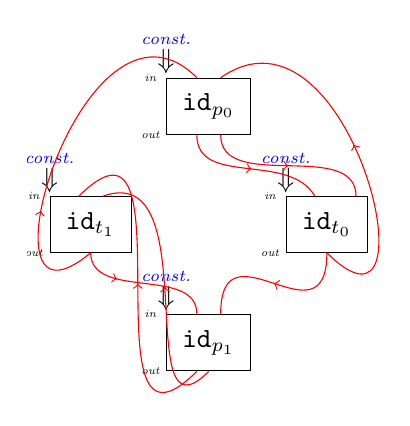
\begin{tikzpicture}      

      % \draw[help lines,step=8pt] (-2.4cm,1cm) grid (2.4cm,-3.7cm);
      \clip (-2.3cm, 1cm) rectangle (2.2cm,-3.7cm);
      
      % P0 Component + I/O
      
      \node[draw, black, inner sep=2mm] (compP0) {$\mathtt{id}_{p_0}$};
      \node at ($(compP0.north west)-(.2,0)$) {\fontsize{4}{6}\selectfont\itshape in};
      \node at ($(compP0.south west)-(.2,0)$) {\fontsize{4}{6}\selectfont\itshape out};
      \node (compP0arrows) at ($(compP0.north west)+(0,2mm)$) {$\Downarrow$};
      \node (labelP0arrows) at ($(compP0arrows.north)$){\ssmall\it \textcolor{blue}{const.}};
      
      % T0 Component + I/O
      
      \node[draw, black, inner sep=2mm] (compT0) at ($(compP0)+(1.5,-1.5)$) {$\mathtt{id}_{t_0}$};
      \node at ($(compT0.north west)-(.2,0)$) {\fontsize{4}{6}\selectfont\itshape in};
      \node at ($(compT0.south west)-(.2,0)$) {\fontsize{4}{6}\selectfont\itshape out};
      \node (compT0arrows) at ($(compT0.north west)+(0,2mm)$) {$\Downarrow$};
      \node (labelT0arrows) at ($(compT0arrows.north)$){\ssmall\it \textcolor{blue}{const.}};            

      % P1 Component + I/O
      
      \node[draw, black, inner sep=2mm] (compP1) at ($(compT0)-(1.5,1.5)$) {$\mathtt{id}_{p_1}$};
      \node at ($(compP1.north west)-(.2,0)$) {\fontsize{4}{6}\selectfont\itshape in};
      \node at ($(compP1.south west)-(.2,0)$) {\fontsize{4}{6}\selectfont\itshape out};
      \node (compP1arrows) at ($(compP1.north west)+(0,2mm)$) {$\Downarrow$};
      \node (labelP1arrows) at ($(compP1arrows.north)$){\ssmall\it \textcolor{blue}{const.}};
      
      % T1 Component + I/O
      
      \node[draw, black, inner sep=2mm] (compT1) at ($(compP1)+(-1.5,1.5)$) {$\mathtt{id}_{t_1}$};
      \node at ($(compT1.north west)-(.2,0)$) {\fontsize{4}{6}\selectfont\itshape in};
      \node at ($(compT1.south west)-(.2,0)$) {\fontsize{4}{6}\selectfont\itshape out};
      \node (compT1arrows) at ($(compT1.north west)+(0,2mm)$) {$\Downarrow$};
      \node (labelT1arrows) at ($(compT1arrows.north)$){\ssmall\it \textcolor{blue}{const.}};


      % INTERCONNECTIONS

      \draw ($(compP0.north)+(1ex,0)$) edge[red,-<-=.5,out=35,in=-45,looseness=2] ($(compT0.south)$);
      \draw ($(compP0.south)+(1ex,0)$) edge[red,->-=.5,out=-90,in=90] ($(compT0.north east)-(1ex,0)$);
      \draw ($(compP0.south)+(-1ex,0)$) edge[red,->-=.5,out=-90,in=120] ($(compT0.north)-(1ex,0)$);
      \draw ($(compT0.south)$) edge[red,->-=.5,out=-90,in=90,looseness=2] ($(compP1.north)+(1ex,0)$);
      \draw ($(compP1.south)-(1ex,0)$) edge[red,->-=.5,out=-135,in=45,looseness=2] ($(compT1.north)-(1ex,0)$);
      \draw ($(compP1.south)$) edge[red,->-=.5,out=-135,in=20,looseness=1.4] ($(compT1.north)+(1ex,0)$);
      \draw ($(compT1.south)$) edge[red,->-=.3,out=-90,in=90] ($(compP1.north)-(1ex,0)$);
      \draw ($(compT1.south)$) edge[red,->-=.3,out=-140,in=135,looseness=2] ($(compP0.north)-(1ex,0)$);
    \end{tikzpicture}
  };

  \node(vhdllabel) at ($(vhdl.south)-(0,.3)$) {$\mathcal{H}$-VHDL top-level design};
  
  \draw (pn.east)
  edge[double, ->, thick]
  node[yshift=1em] {\ssmall Transformation}
  ($(vhdl.west)-(.2,0)$);
  
\end{tikzpicture}

\end{document}